
\section{Digital Communication}

For this section two Quadrature Amplitude Modulation (QAM) techniques were used, \textbf{Quadrature Phase-Shift Keying (QPSK)} and \textbf{16-QAM}. This process involved generating a random stream of bits, modulating them into \textbf{QPSK} and \textbf{16-QAM} symbols and simulating their transmission through GNU Radio. In the simulation the effects of non-linear Power Amplifier (PA) and Low Noise Amplifier (LNA) were simulated as well as the noise of a Additive White Gaussian Noise (AWGN) channel.

\subsection{Digital Modulation}

\label{ssec:modulations}
\textbf{QPSK} places four equally spaced points on the unit circle:
\[
s_k = e^{j\frac{\pi}{2}\left(k+\tfrac12\right)}, \qquad k\in\{0,1,2,3\}.
\]

Figure \ref{fig:QPSK_const}, shows the mapping in the cartesian plane.


The mapper groups the encoded bit stream into two-bit tuples $(b_1,b_0)$, converts each tuple to an integer index $(k =2b_1+b_0)$ and outputs \(s_k\).

The theoretical bit-error probability for QPSK in an AWGN channel is given by Equation \ref{eq:probErrQPSK}.
\begin{equation}
  P_b^{\text{QPSK}} = Q\left(\sqrt{2\frac{E_b}{N_0}}\right)\text{\cite{Work_TAC2025}}
  \label{eq:probErrQPSK}
\end{equation}

For \textbf{QPSK}, demodulation is performed by simply de-mapping the bit values.


With \textbf{16-QAM} a $4\times4$ square constellation was used. What changes comparing to the previous mapping approach is the fact that the amplitude also changes and for this specific mapping the phase and amplitude will not change consistently. The symbol position in the cartesian frame will be:
\[
I,R \in \{\pm3,\;\pm1\}
\]

For \textbf{16-QAM} the theoretical \textbf{BER} for an AWGN channel with gray mapping is given by Equation \ref{eq:probErr16QAM}.

\begin{equation}
  P_b^{\text{16QAM}} \approx \frac{3}{4}\cdot Q\left(\sqrt{\frac{4}{5}\frac{E_b}{N_0}}\right)\text{\cite{Work_TAC2025}}
  \label{eq:probErr16QAM}
\end{equation}


The constellation points are labelled with \emph{Gray coding}, thus every nearest neighbour differs in \emph{exactly one} bit, this will minimize \textbf{BER}, since the most likely symbol error produces only one wrong bit. Figure \ref{fig:16QAM_const}, shows how the codes are mapped.


\begin{comment}
    
\begin{figure}[H]
    \centering
    \includegraphics*[width=0.8\textwidth]{Images/Const_QPSK.png}
    \caption{QPSK Constellation}
    \label{fig:QPSK_const}
\end{figure}

\begin{figure}[H]
    \centering
    \includegraphics*[width=0.8\textwidth]{Images/Const_16QAM.png}
    \caption{16-QAM Constellation}
    \label{fig:16qam_const}
\end{figure}

\end{comment}

\begin{figure}[H]
    \centering
    \begin{subfigure}[t]{0.5\textwidth}
        \centering
        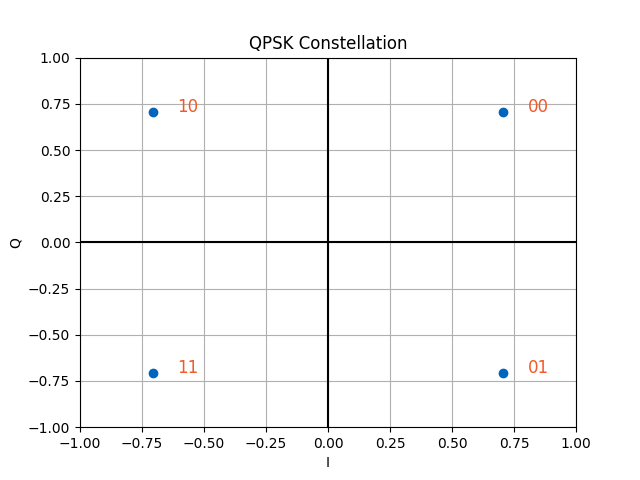
\includegraphics[width=\textwidth]{Images/Const_QPSK.png}
        \caption{QPSK Constellation.}
        \label{fig:QPSK_const}
    \end{subfigure}%
    \begin{subfigure}[t]{0.5\textwidth}
        \centering
        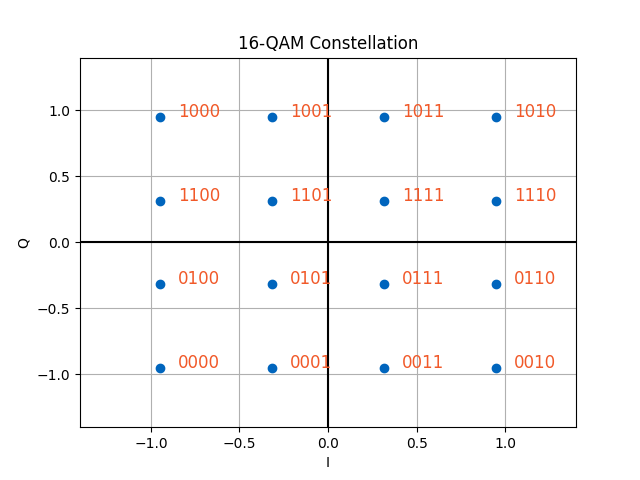
\includegraphics[width=\textwidth]{Images/Const_16QAM.png}
        \caption{16-QAM Constellation.}
        \label{fig:16QAM_const}
    \end{subfigure}
    \caption{Digital Modulation Constellations.}
    \label{fig:Const}
\end{figure}

\subsection{GNU Radio Implementation}

The GNU Radio design aims to simulate an RF (radio frequency) QAM communication 
between a transmitter and a receiver through an AWGN channel.
This simulation also includes non linear elements from the power amplifiers used 
in these circuits [Fig.\ref{fig:PA_non_lin}], and channel imperfections, such 
as signal attenuatin that occurs in the channel [Fig.\ref{fig:Gnu_Channel}].

\subsubsection{IQ Modulation}

The transmitter modulates two different signals effectivly transfering the original signals 
from the original baseband to the channel frequency (Fc). These signals are modulated 
with a \ang{90} angle phase shift between them [Fig.\ref{fig:IQMod_Diagram} and \ref{fig:GNU_IQMod}].
This means the modulated signals are in quadrature with each other, thus allowing the 
transmitter to transmit both signals at the same time without them interfering with each 
other.

\begin{figure}[H]
    \centering
    \includegraphics*[width=0.7\textwidth]{Images/IQ_Mod_Diagram.png}
    \caption{IQ Modulator Block Diagram}
    \label{fig:IQMod_Diagram}
\end{figure}

\begin{figure}[H]
    \centering
    \includegraphics*[width=0.9\textwidth]{Images/GNU_Digital_IQMod.png}
    \caption{GNU IQ Modulator}
    \label{fig:GNU_IQMod}
\end{figure}

On the receiver's side, the same method is applied to demodulate the received signal and 
recover both the original signals, [Fig.\ref{fig:IQDeMod_Diagram} and  
\ref{fig:GNU_IQDemod}]. 

\begin{figure}[H]
    \centering
    \includegraphics*[width=0.7\textwidth]{Images/IQ_Demod_Diagram.png}
    \caption{IQ De-Modulator Block Diagram}
    \label{fig:IQDeMod_Diagram}
\end{figure}

\begin{figure}[H]
    \centering
    \includegraphics*[width=0.9\textwidth]{Images/GNU_Digital_IQDemod.png}
    \caption{GNU IQ De-Modulator}
    \label{fig:GNU_IQDemod}
\end{figure}

Since the received signals are in quadrature with each other demodulating them with the 
same signal used on the transmitter, (a signal with the same frequency and pahse as 
used in the transmitter to modulate), the original signal is recovered.

\subsubsection{Nonideal simulation elements}

\textcolor{red}{Arranjar outro titulo e texto a explicar 3 ordem de nao lin, limitacoes que vao apararecer e dizer que pro lNA é mais do mesmo}

The cahnnel used for RF communications, in the real world, attenuates the transmitted signal 
and adds some white noise as well. 

\paragraph{}
These effects are replicated in the simulation using a constant value multiplier in 
the channel with a constant value smaller than 1, and a adding a the transmitted signal to 
a signal produced by the signal generated by a white noise source, [Fig.\ref{fig:Gnu_Channel}].

\begin{figure}[H]
    \centering
    \includegraphics*[width=0.9\textwidth]{Images/GNU_Channel.png}
    \caption{GNU Radio Channel}
    \label{fig:Gnu_Channel}
\end{figure}
\textcolor{red}{Dizer que o noise é adicionado antes da atenuaçao para manter o SNR mais facil de quantificar}

To counteract the undesired effects of the channel an amplifier is introduced, both 
in the transmitter and the receiver.

\paragraph{}
Idealy these amplifiers would provide a linear gain to the signal, however the components 
used to create these amplifiers are ideal, in which case, the real amplifiers add a nonlinear 
component the signal gain.

Assuming the gain of these amplifiers can be expressed as a function of the input signal, 
then the output of these amplifiers can be described as \(y(t) = Amp(x(t))\), then using 
taylor series' the output can be approximated to the result fo Equation \ref{eq:Taylor_series_approx}.

\begin{equation}
    y(t) = \sum_{n=0}^{\infty} \frac{\partial^n Amp(x_0)}{\partial x^n \cdot n!} \cdot (x - x_0)^n \leftrightarrow y(t) \approx a_1x(t) + a_2{x(t)}^2 + a_3{x(t)}^3
    \label{eq:Taylor_series_approx}
\end{equation}

Where \(x_0\) is the dc operating point voltage of the input, was set to 0 to simplify calculations, \(a_n\) is the value of the nth derivative with respect to \(x(t)\) evaluated at \(x(t) = 0\) divided by the number of derivatives taken.

The second-order nonlinearity, the second derivative, will produce a tone with double the frequency of the fundamental, causing harmonic distortion. However the most important effect is the third order effect, which has effects on the third harmonic as well as in the fundamental, this effect is seen as a compression of the signal.   

\paragraph{}
To simplify the GNU Radio schematic only the 3 higher order Taylor series' components were 
used, these are also the most influential components in the real circuit. The GNU Radio 
circuit is shown in Figure \ref{fig:PA_non_lin}. Because of this model limitations, when the third order effects are larger than the linear gain, the signal will expand instead of compress, and will instead have an opposite phase.

\begin{figure}[H]
    \centering
    \includegraphics*[width=0.9\textwidth]{Images/PA_non_lin.png}
    \caption{GNU Radio PA non Linear}
    \label{fig:PA_non_lin}
\end{figure}

\subsection{Performance Analysis}

The primary goal was to evaluate the system's performance by measuring the Bit Error Rate (BER) as a function of the Signal-to-Noise Ratio (SNR) in an AWGN channel.

A random bitstream of $3 \times 10^6$ bits was generated using \texttt{Gen\_symbs.py} \textcolor{red}{Meter cite aos anexos?}. This stream was modulated and fed into the GNU Radio simulation. At the receiver, the \texttt{Read\_Output.py} script was used to read the output files and calculate BER.

Finally with BER values were plotted against the theoretical performance curves, Equations \ref{eq:probErrQPSK} and \ref{eq:probErr16QAM}, for both modulation schemes. As shown in Figure \ref{fig:BER_SNR_a3_0}, in this figure there were no non-linear effects simulated.

\begin{figure}[H]
    \centering
    \includegraphics*[width=0.9\textwidth]{Images/BER_SNR_a3_0.png}
    \caption{BER vs $E_b/N_0$}
    \label{fig:BER_SNR_a3_0}
\end{figure}

The results in Figure \ref{fig:BER_SNR_a3_0} clearly validate our simulation.

\textbf{QPSK} BER points (shown in orange) align almost perfectly with the theoretical QPSK performance curve. This confirms that the simulation chain, including the noise model and demodulator, is functioning correctly.

\textbf{16-QAM} similarly, the simulated 16-QAM data (in Blue) closely follows its theoretical curve.


\begin{comment}
    
\subsubsection{Results Discussion}

\begin{itemize}
    \item \textbf{QPSK:} The simulated BER points (shown in blue) align almost perfectly with the theoretical QPSK performance curve. This confirms that the simulation chain, including the noise model and demodulator, is functioning correctly.

    \item \textbf{16-QAM:} Similarly, the simulated 16-QAM data (in orange) closely follows its theoretical curve.

    \item \textbf{Performance Trade-off:} The graph clearly illustrates the fundamental trade-off between data rate and noise immunity. To achieve the same Bit Error Rate, 16-QAM requires a significantly higher SNR than QPSK. For example, to achieve a BER of $10^{-3}$ (0.1\%), QPSK requires an SNR of approximately 7 dB, while 16-QAM requires approximately 10.5 dB. This demonstrates that while 16-QAM can transmit twice the amount of data per symbol, it is much more susceptible to noise.
\end{itemize}

\end{comment}